\documentclass{article}
\usepackage[utf8]{inputenc}
\usepackage[margin=2.5cm]{geometry}
\usepackage{amsmath}
\usepackage{graphicx}
\usepackage{physics}
\usepackage{caption}
\usepackage{subcaption}
\usepackage{comment}
\title{notes}
\author{zhongshan1111 }
\date{May 2022}
\setlength\parindent{0pt}

\begin{document}



\section{Technical Background}
K-means clustering is an unsupervised Machine Learning (ML) protocol whose main goal is to classify datasets into K clusters. The term “k-means” was first used by James MacQueen in 1967, and published as a journal article in 1982. K-means clustering can minimize within cluster variances, the problem is computationally difficult (NP-hard) and the time complexity of the algorithm is specified by O(LNpK), where L = number of iterations taken to form clusters, N = number of datapoints, p = dataset dimension, K = centroids.\\

Clustering is the process of dividing the datasets into groups such that points in the same group are as similar as possible, and points in different groups are as dissimilar as possible. The k-means algorithm finds groups with the number of groups represented by the variable $K$. The algorithm works in an iterative manner to assign each data point to one of the k groups based on the features that are provided. \\

Fig.\ref{fig:kmeansclassica} give an example of how K-means to divide the similar datasets into one group, in this case K=3
\begin{figure}[h]
    \centering
    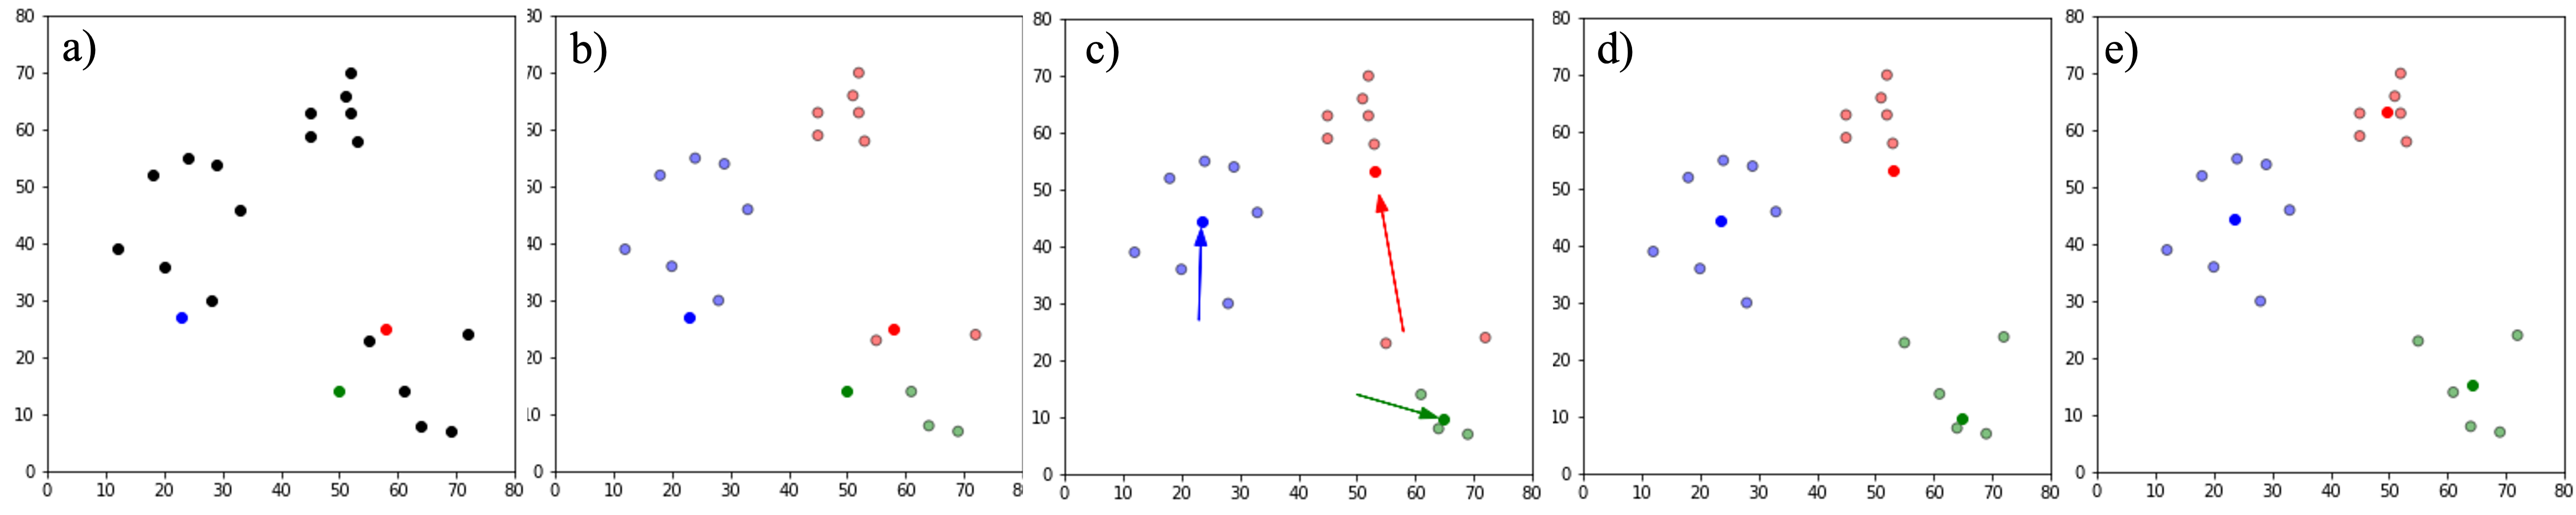
\includegraphics[width=1\textwidth]{figure/kmeansclassical.png}
    \caption{Some random 2D training data points are plotted with black dots in a), three random points are chosen to be the cluster centroids. b) Assign the training data points to the selected clusters. c) Calculate average and update the cluster centroids. d)Repeat data assignment in figure b). e) Repeat figure b), c) and d) until final clusters e) are reached.}
    \label{fig:kmeansclassica}
\end{figure}

A general way of doing the K-means algorithm is usually summarized in the following steps:
\begin{itemize}
    \item Initialize uniformly distributed cluster centroids $c_j$ which are randomly selected from the data setsInitialize uniformly distributed cluster centroids $c_j$ which are randomly selected from the data sets.
    \item For each $c_j$, the chosen metric is evaluated. For example, in simpler cases, the distance between each training data point and selected cluster centroids $c_j$ is evaluated.
    \item New clusters $C_j$ are defined by assigning training data to the nearest cluster centroids $c_j$.
    \item New cluster centroids are updated
    \item Repeat steps 3 to 5 are repeated depending on the resource constraints
\end{itemize}
In the second step, the Euclidean distance between cluster centroids and training data point need to be efficiently sampling and estimating, however it becomes exponentially difficult as number of variables (features) of each data point increase. Therefore, implement a computationally cheap quantum algorithm to calculate Euclidean distance is helpful.\\

In this project, our team proposed a hybrid algorithm which contains classical calculation to calculate cluster centroids and assigns features and using quantum circuit to compute Euclidean distance. 

\section{Hybrid K-means clustering}
The hybrid K-means clustering algorithm contains quantum circuit to calculate the Euclidean distance between the cluster centroids and the training data points, and classical method to assign and update cluster centroids. The work flow of the hybrid K-means clustering is presented in Fig. \ref{fig:qkmeans}

\begin{figure}[h]
    \centering
    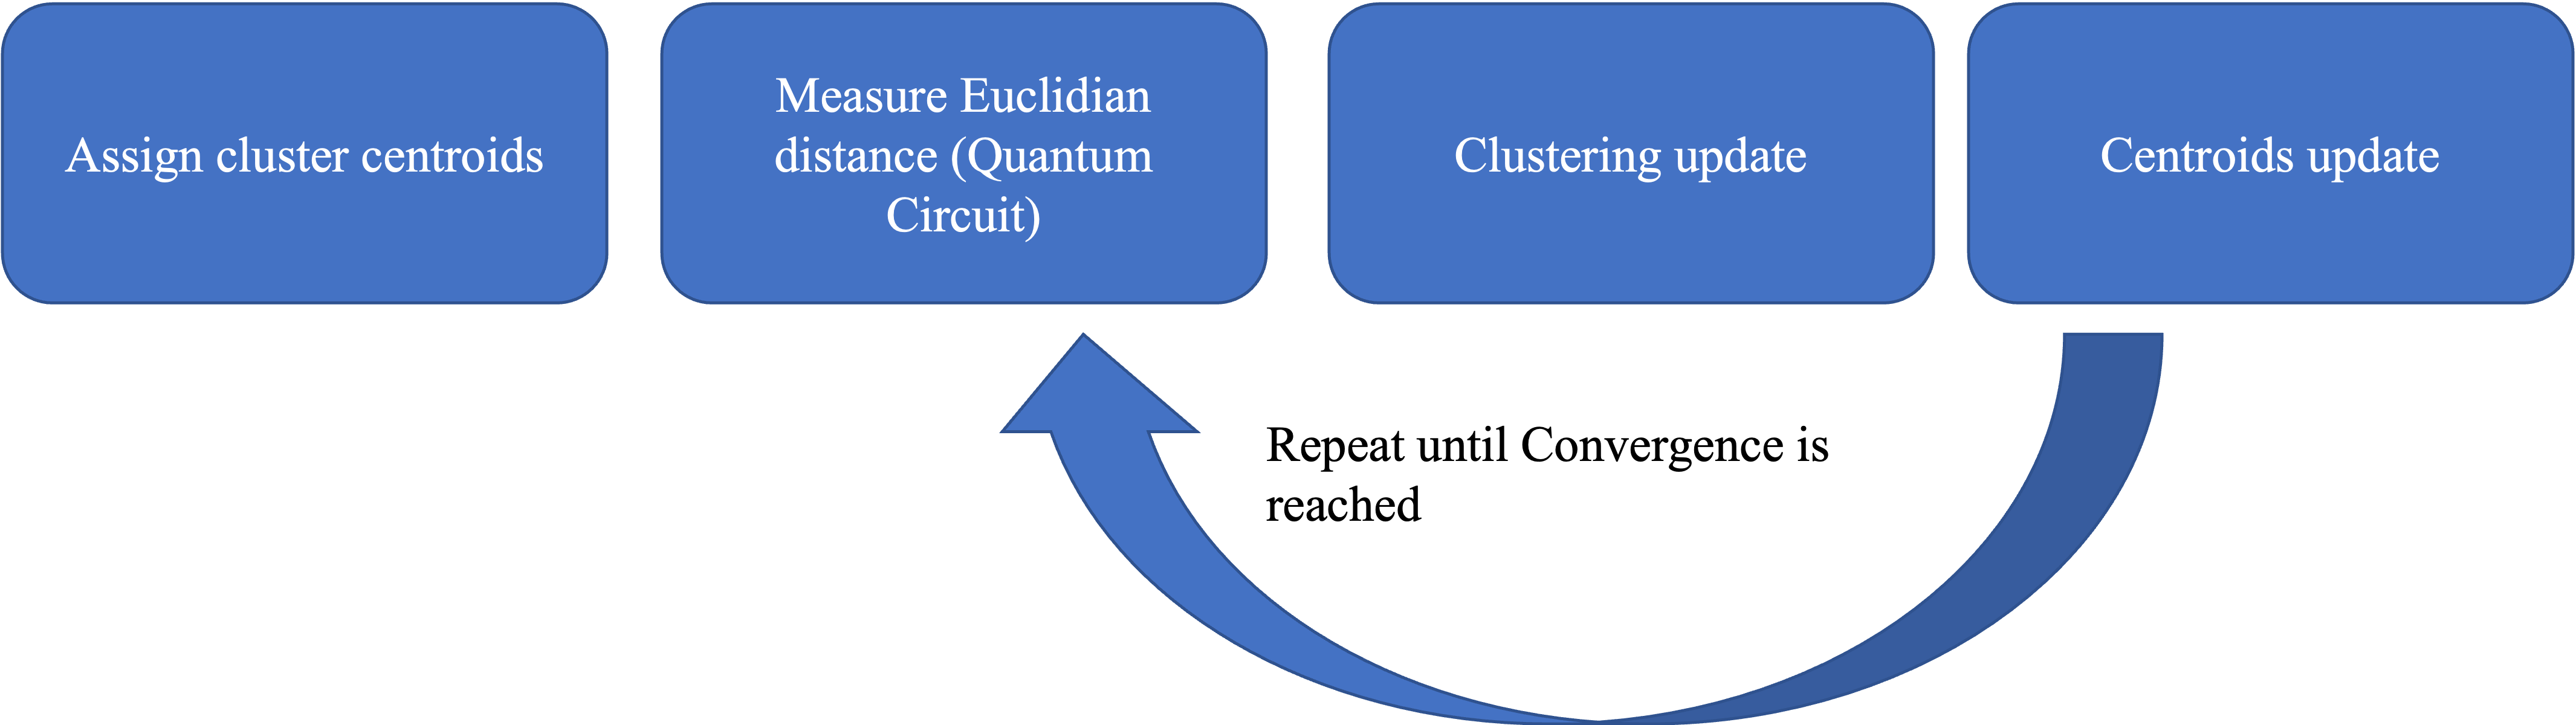
\includegraphics[width=0.8\textwidth]{figure/quantum Kmeans flow.png}
    \caption{: A flow chart of how the hybrid K-means clustering algorithm works in our system.}
    \label{fig:qkmeans}
\end{figure}

The first step is to randomly assign the cluster centroids, however in order to perform quantum computing, we need to convert the classical centroids into quantum states and here we use the amplitude embedded method. Suppose we have a centroid $x$ with $n$ dimensions (features) which can be written in the form of a vector $x=[x_1,x_2,x_3,... x_n]$ where $x_j (j\in n)$ is the feature. With the the amplitude embedding, the classical information can be mapped into Hilbert Space in a form of
\begin{equation}
\ket{a}=\frac{1}{|X|}\sum_{i=1}^nx_i\ket{x_i}
\end{equation}
where $|X|$ is the normalization factor, $\ket{x_i}$ is the quantum state which is in bit string configuration and $x_i$ is the features of the cluster centroids. We can also apply the similar transformation technique to the training data points $y$ and we have 
\begin{equation}
\ket{b}=\frac{1}{|Y|}\sum_{i=1}^ny_i\ket{y_i}
\end{equation}
After forming the quantum states the question of finding Euclidian distance between two classical points are mapped into finding the distance between two quantum states $\ket{a}$ and $\ket{b}$. 
Firstly, we generate two with $\ket{a}$, $\ket{b}$ and an ancillary qubit
\begin{align}
    \ket{\psi}&=\frac{1}{\sqrt{2}}(\ket{0}\otimes\ket{a}+\ket{1}\otimes\ket{b})\\
    \ket{\phi}&=\frac{1}{Z}(|a|\ket{0}+|b|\ket{1})
\end{align}
where $Z= \sqrt{|a|^2+|b|^2}$ is the normalization constant. Next step, we introduce the \textbf{swap test} [2] to computing the distance. The swap test aims to apply a controlled swap gate to $\ket{\psi}$ and $\ket{\phi}$ which allows us to experimentally determine the overlap between the two states $|\bra{\psi}\ket{\phi}|^2$, this will be integral in calculating the Euclidean distance. The initial state for quantum computing is
\begin{equation}
\ket{S_0}=\ket{0}\otimes\ket{\psi}\otimes\ket{\phi}
\end{equation}
Then we apply a Hadamard gate on the ancillary qubit to make a superposition state
\begin{equation}
\ket{S_1}=\frac{1}{\sqrt{2}}(\ket{0}\otimes\ket{\psi}\otimes\ket{\phi}+\ket{1}\otimes\ket{\psi}\otimes\ket{\phi})
\end{equation}
The controlled SWAP gate is then applied to swap  $\ket{\psi}$ and $\ket{\phi}$ conditioned on the ancillary qubit, this result in
\begin{equation}
    \ket{S_2}=\frac{1}{\sqrt{2}}(\ket{0}\otimes\ket{\psi}\otimes\ket{\phi}+\ket{1}\otimes\ket{\phi}\otimes\ket{\psi})
\end{equation}
Another Hadmard gate is placed on the ancillary qubit at the end gives the result
\begin{equation}
    \ket{S_3}=\frac{1}{2}\ket{0}\otimes(\ket{\psi}\otimes\ket{\phi}+\ket{\phi}\otimes\ket{\psi})+\frac{1}{2}\ket{1}\otimes(\ket{\phi}\otimes\ket{\psi}-\ket{\psi}\otimes\ket{\phi})
\end{equation}
Finally, we measure state $\ket{S_3}$ with the ancillary qubit $\ket{0}$, the probability $P(0)$ is 
\begin{equation}
    P(0)=|\bra{0}\ket{S_3}|^2=\frac{1}{2}+\frac{1}{2}|\bra{\psi}\ket{\phi}|^2
\end{equation}
The final Euclidean distance is
\begin{equation}
    |a-b|^2=Z(4P(0)-2)
\end{equation}


\section*{Reference}
[1] A. Sarma, R. Chatterjee, K. Gili, and T. Yu, “Quantum unsupervised and supervised learning on superconducting processors,” Quantum Information and Computation 20 (2019), 10.48550/arXiv.1909.04226.\\

[2] M. Kang and J. Heo and S. Choi and S. Moon and S. Han (2019), Implementation of SWAP test for two unknown states in photons via cross-Kerr nonlinearities under decoherence effect, Scientific Reports Vol. 9., 10.1038/s41598-019-42662-4.

\end{document}
